% Kommentierte und erweiterte Quelldatei zu Video 02 der LaTeX
% Tipps-Tricks-Techniken Serie von Thomas Erben
% (siehe )

\documentclass[12pt,a4paper]{scrartcl}

\usepackage[ngerman]{babel}
\usepackage[utf8]{inputenc}
\usepackage[T1]{fontenc}

\usepackage{graphicx}     % Zum Einbinden von Figuren nötig

% Beachten Sie bei dem folgenden Befehl dass das Argument
% 'figuren/' in ein zweites geschweiftes Klammernpaar
% eingebunden ist. Auch der '/' am Ende von 'figuren'
% ist wesentlich!
\graphicspath{{figuren/}}
  % Figuren befinden sich im Verzeichnis
  % 'figuren' (Unterverzeichnis der
  % LaTeX Quelltexte.

% Das folgende Paket ist notwendig, wenn man 'Unterfiguren'
% referenzieren möchte
\usepackage[list=true]{subcaption}
  
% Kommando zum einfach Referenzieren von Figuren
\newcommand{\figref}[1]{Figur~\ref{#1}}

\begin{document}
%
\tableofcontents
\listoffigures
%
\section{Figuren nebeneinander setzen}
Im folgenden zeige ich zwei prinzipielle Möglichkeiten, Figuren
nebeneinander zu setzen. Die Möglichkeiten unterscheiden sich darin,
ob die beiden Figuren separat referenziert werden sollen oder nicht.
%
\subsection{Figuren müssen nicht separat referenziert werden}
Diese Möglichkeit wurde schon in Video 16 der \LaTeX-Einführungsserie
besprochen. \figref{fig:quad_recht} zeigt ein Quadrat und ein Rechteck.
%
\begin{figure}[ht]
  \centering
  % Wir fassen zwei Figuren zu einer zusammen. Damit so nebeneinander
  % gesetzt werden darf die Gesamtbreite der Figuren '\textwidth'
  % nicht überschreiten.
  \includegraphics[width=0.49\textwidth]{quadrat}   
  \includegraphics[width=0.49\textwidth]{rechteck}  
  \caption[Geometrische Figuren (zwei nebeneinander)]{Quadrat (links)
    und Rechteck (rechts)}
  \label{fig:quad_recht}
\end{figure}
%
Wie im Video besprochen, zeige ich in \figref{fig:drei_fig} und
\figref{fig:vier_fig} noch Möglichkeiten, drei und vier Figuren
zusammenzufassen.
%
\begin{figure}[ht]
  \centering
  \includegraphics[width=0.31\textwidth]{quadrat}  
  \includegraphics[width=0.31\textwidth]{rechteck}
  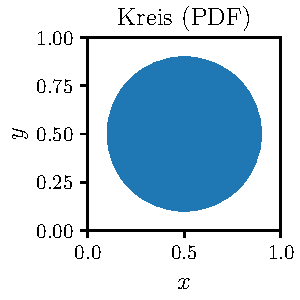
\includegraphics[width=0.31\textwidth]{kreis}  
  \caption[Geometrische Figuren (drei nebeneinander)]{Quadrat
    (links), Rechteck (Mitte) und Kreis (rechts)}
  \label{fig:drei_fig}
\end{figure}
%
\begin{figure}[ht]
  \centering
  \includegraphics[width=0.3\textwidth]{quadrat}  
  \includegraphics[width=0.3\textwidth]{rechteck}

  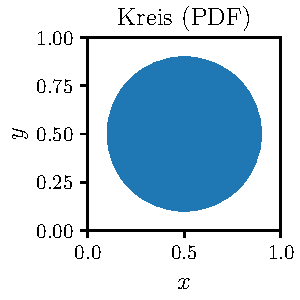
\includegraphics[width=0.3\textwidth]{kreis}  
  \includegraphics[width=0.3\textwidth]{ellipse}  
  \caption[Geometrische Figuren (vier als Quadrat angeordnet)]{Quadrat
    (links oben), Rechteck (rechts oben), Kreis (links unten) und
    Ellipse (rechts unten)}
  \label{fig:vier_fig}
\end{figure}
%
\subsection{Figuren sollen separat referenziert werden}
%
\figref{fig:quad_recht_subfigure} zeigt Quadrat und Rechteck als
Unterfiguren, die separat referenziert werden können.
\figref{subfig:quad} ist das Quadrat und \figref{subfig:recht} das Rechteck.
\begin{figure}[ht]
  %
  \begin{subfigure}[t]{0.49\textwidth}
    \centering
    \includegraphics[width=\textwidth]{quadrat}
    \caption[Quadrat]{Ein Quadrat. Ein Quadrat ist ein \emph{spezielles}
      Rechteck, bei dem die Breite und die Höhe gleich sind.}
    \label{subfig:quad}
  \end{subfigure}
  % 
  \begin{subfigure}[t]{0.49\textwidth}
    \centering
    \includegraphics[width=\textwidth]{rechteck}
    \caption[Rechteck]{Ein Rechteck}
    \label{subfig:recht}
  \end{subfigure}
  %
  \caption[Geometrische Figuren (Unterfiguren)]{Die Figuren Quadrat und Rechteck als Unterfiguren}
  \label{fig:quad_recht_subfigure}
\end{figure}
%
\end{document}
